\documentclass[10pt,a4paper]{article}
\usepackage[margin=1.5cm]{geometry}
\usepackage{graphicx,amsmath,xcolor,enumitem,booktabs}
\usepackage[most]{tcolorbox}
\usepackage[T1]{fontenc}
\usepackage{lmodern,microtype}
\usepackage{titlesec,multicol}
\usepackage[hidelinks]{hyperref}

\definecolor{acc}{RGB}{15,106,74}
\definecolor{warn}{RGB}{185,60,40}
\titleformat{\section}{\large\bfseries\color{acc}}{\thesection}{0.6em}{}
\titlespacing*{\section}{0pt}{8pt}{4pt}
\setlength{\parindent}{0pt}
\setlength{\parskip}{3pt}

% Numbered item: \lab{n}{Title}{text}
\newcommand{\num}[1]{\tikz[baseline=(c.base)]\node[circle,fill=red!75!black,text=white,inner sep=1.2pt,minimum size=13pt,font=\footnotesize\bfseries](c){#1};}
\usepackage{tikz}
\newenvironment{labels}{\begin{description}[leftmargin=0pt,labelsep=0.4em,itemsep=3pt,parsep=1pt,font=\normalfont]}{\end{description}}
\newcommand{\lab}[2]{\item[\num{#1}\ \textbf{#2}]}
\newcommand{\what}{\textit{What:}\ }
\newcommand{\how}{\textit{How:}\ }
\newcommand{\theory}{\textit{Theory:}\ }
\newtcolorbox{vnote}{colback=warn!6,colframe=warn!70,boxrule=0.5pt,left=4pt,right=4pt,top=2pt,bottom=2pt,fontupper=\small,
  title={\small\bfseries Viva note},coltitle=white,colbacktitle=warn!80,toptitle=1pt,bottomtitle=1pt}
\newtcolorbox{keybox}{colback=acc!5,colframe=acc!70,boxrule=0.5pt,left=4pt,right=4pt,top=2pt,bottom=2pt,fontupper=\small}

\begin{document}

{\LARGE\bfseries\color{acc} SonicVitals: Viva Guide to the Dashboards}\\[2pt]
{\small Every numbered label on the three screenshots, with what it shows, how it is computed and the theory behind it.}

\section*{The project in one paragraph}
SonicVitals is a contactless vital-signs system. An \textbf{ESP32-S3} board carries a camera (GC2145, 240$\times$160 pixels), an
\textbf{INMP441} I$^2$S MEMS microphone and a 0.96'' \textbf{SSD1306 OLED}. The board streams JPEG frames and audio to a laptop
(over Wi-Fi, TCP port 3333). The laptop runs a Python/Flask server that detects the face, extracts skin colour over time
(\textbf{remote photoplethysmography, rPPG}) to estimate heart rate (HR) and respiratory rate (RR), and analyses heart sounds
(\textbf{phonocardiography, PCG}) from the microphone. Results go to the web dashboard and back to the OLED.

\begin{keybox}
\textbf{Core principle of rPPG.} With every heartbeat, more blood enters the skin capillaries. Haemoglobin absorbs light (strongly in
green, less in red), so the skin's reflected colour changes by about 0.1--1\,\% at the heart rate. The eye cannot see it, but the
\emph{average} over thousands of skin pixels makes it measurable. \textbf{Pipeline:} face detection $\rightarrow$ skin ROI mean
(R,\,G,\,B) per frame $\rightarrow$ CHROM colour projection $\rightarrow$ band-pass 0.75--2.5\,Hz $\rightarrow$ Welch spectrum
$\rightarrow$ highest peak $f_0$ $\rightarrow$ HR $=60 f_0$.
\end{keybox}

\begin{vnote}
These three screenshots come from the \textbf{first build} (5 Oct). A few cards in that build showed values produced by fixed
formulas or labels, not measurements; they are marked below with ``\emph{Viva note}''. Say this openly if asked. It shows you
understand your own system, and the current build has already fixed them.
\end{vnote}

% =====================================================================
\section{Dashboard (live monitoring)}
\begin{center}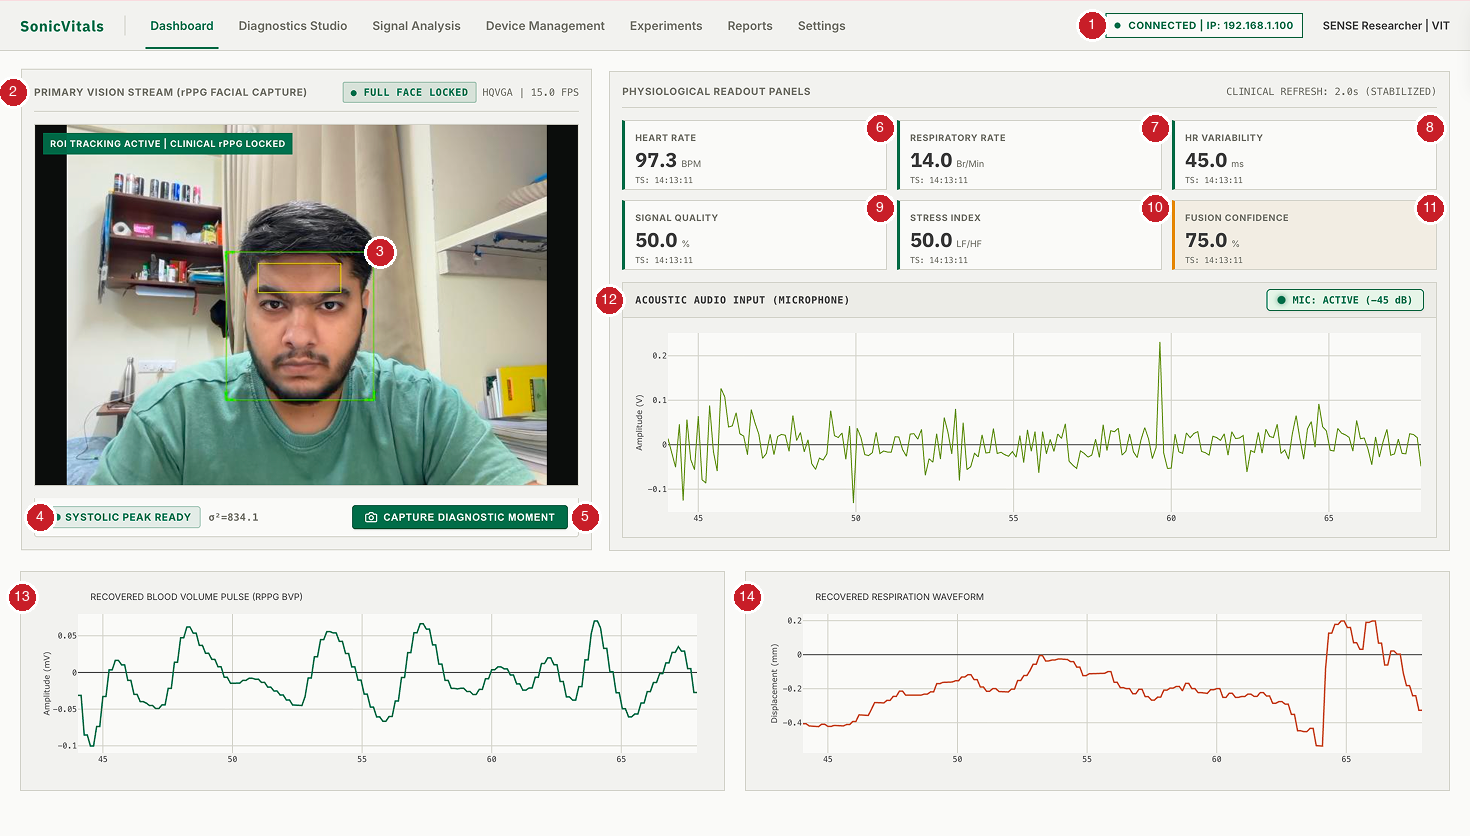
\includegraphics[width=\linewidth]{fig/dash.png}\end{center}

\begin{labels}
\lab{1}{Connection badge.} \what shows whether the host is receiving data from the node. \how the server polls the link; the
badge turns green when frames arrive.
\begin{vnote}``IP 192.168.1.100'' was fixed text in the first build's HTML. The current badge shows the real link
(e.g.\ \texttt{tcp://sonicvitals.local:3333}).\end{vnote}

\lab{2}{Primary vision stream.} \what the live camera picture after processing, served by Flask as an MJPEG stream
(\texttt{/video\_feed}). ``FULL FACE LOCKED'' means the frame passed the five-test face gate (item 3). ``HQVGA'' is the
240$\times$160 resolution. \theory rPPG needs a still, well-lit, fully visible face; anything else adds noise far bigger than the
pulse.
\begin{vnote}``15.0 FPS'' was a fixed label. The real frame rate over Wi-Fi is about 8 frames/s (measured; the dashboard now
shows the measured value).\end{vnote}

\lab{3}{Face box (green) and forehead ROI (yellow).} \what where the face was found and which skin patch gives the pulse.
\how \textbf{Viola--Jones Haar cascade} (OpenCV): the image is converted to grey and histogram-equalised, then scanned with
rectangular Haar features evaluated quickly through an \emph{integral image}. AdaBoost-selected features are arranged in a
\emph{cascade}, so non-face windows are rejected early. The box is smoothed over frames to stop jitter. \textbf{Five-test gate}:
(1)~face not touching the edges, (2)~face size 20--88\,\% of the frame width, (3)~aspect ratio 0.65--1.30 (not turned),
(4)~all ROIs inside the image, (5)~enough light (cheek brightness $>15$) and similar left/right brightness. Only frames that pass
enter the analysis. \textit{Current build:} forehead \emph{plus both cheeks} (more skin pixels means less noise).

\lab{4}{``Systolic peak ready'' and $\sigma^2 = 834.1$.} \what $\sigma^2$ is the \textbf{sharpness} of the best frame in the last
8\,s: the variance of the Laplacian (2nd-derivative filter) of the grey image. A blurred or moving image has weak edges, so a low
variance; higher means sharper. The sharpest frame is kept for the colour analysis (Diagnostics Studio).
\begin{vnote}``Systolic peak'' was set when the latest green value was above its 10-frame mean. That is not a reliable systole
detector (in systole green \emph{drops}), so it was removed from the current build.\end{vnote}

\lab{5}{Capture Diagnostic Moment.} \what sends the sharpest gated frame to \texttt{/api/capture\_diagnostic}, which computes
the colour indices shown in the Diagnostics Studio.

\lab{6}{Heart rate (97.3 BPM).} \how ROI means $R,G,B$ are buffered with timestamps and resampled to a uniform 15\,Hz grid.
\textbf{CHROM} (de Haan \& Jeanne, 2013): each channel is divided by its mean over a short window (removes light intensity),
then
\[ X = 3R_n - 2G_n,\quad Y = 1.5R_n + G_n - 1.5B_n,\quad S = X - \alpha Y,\ \ \alpha=\sigma_X/\sigma_Y . \]
$X$ and $Y$ both contain the motion/specular component, so subtracting $\alpha Y$ cancels it and leaves the pulse $S$. $S$ goes
through a 3rd-order \textbf{Butterworth band-pass} 0.75--2.5\,Hz (45--150\,BPM), run forwards and backwards (\texttt{filtfilt},
zero phase). A \textbf{Welch} spectrum (Signal Analysis, item 7) gives the peak $f_0$; $\text{HR}=60 f_0$. The display is refreshed every
2\,s and smoothed with an exponential moving average (EMA). Normal resting adult range: 60--100\,BPM.

\lab{7}{Respiratory rate (14.0 br/min).} \theory breathing slowly modulates the skin signal (changes in venous return, chest/head
movement and light angle): \emph{respiratory-induced intensity variation}. \how the green channel is band-passed
0.15--0.40\,Hz (9--24 breaths/min) and the spectral peak $f_r$ gives $\text{RR}=60f_r$. Normal adult: 12--20 br/min.
\textit{Current build:} RR is shown only if the peak holds $\geq 50\,\%$ of the low-frequency power (otherwise ``--'').

\lab{8}{HR variability (45.0 ms).} \theory HRV is the beat-to-beat variation of the interval between heartbeats (IBI). Standard
time-domain measure: $\text{RMSSD}=\sqrt{\tfrac{1}{N-1}\sum (IBI_{i+1}-IBI_i)^2}$; typical resting values 20--60\,ms.
\begin{vnote}In the first build this card was \emph{not measured}: it was $55+0.4(\text{SQI}-75)$, and with SQI $=50$ that gives
exactly 45.0. The current build computes real RMSSD from heart-sound beat times (needs $\geq 20$ clean intervals), else ``--''.\end{vnote}

\lab{9}{Signal quality (50.0 \%).} \what how dominant the cardiac peak is. First build: $\min(99,\max(50,\,160\,P_\text{peak}/P_\text{band}))$.
\textbf{50.0 is the floor}, meaning the peak held $\leq 31\,\%$ of band power: a \emph{weak} signal at that moment.
\textit{Current build:} spectral concentration $Q$ (power within $\pm0.1$\,Hz of $f_0$ divided by band power), with no clamp.

\lab{10}{Stress index (50.0, labelled LF/HF).} \theory the real LF/HF index is the ratio of HRV spectral power at
0.04--0.15\,Hz (sympathetic + parasympathetic) to 0.15--0.4\,Hz (parasympathetic); it needs minutes of accurate beat times.
\begin{vnote}It was not LF/HF: it was $50-0.5(\text{HRV}-45)$, which is 50.0 when HRV is 45.0. Removed in the current build.\end{vnote}

\lab{11}{Fusion confidence (75.0 \%).} \theory \emph{sensor fusion} combines the camera HR and the microphone HR, weighted by
their quality. \textit{Current build:} $\text{HR}=(w_o\,\text{HR}_o + w_a\,\text{HR}_a)/(w_o+w_a)$ if the two agree within
8\,BPM; otherwise the higher-quality channel is used and a conflict is flagged.
\begin{vnote}First build: $\max(75,\,1.05\cdot\text{SQI})$, so 75.0 is the floor value, not a measured confidence.\end{vnote}

\lab{12}{Acoustic input (MIC $-45$ dB).} \what live microphone waveform. $-45$\,dB $=20\log_{10}(\text{peak
amplitude})$, i.e.\ dB relative to full scale (dBFS); quiet input. Tall spikes are clicks or speech.
\theory heart sounds S1 (valves closing at the start of systole) and S2 (end of systole) lie at 20--150\,Hz. \textit{Current build:}
the ESP32's INMP441 is used. Audio is band-passed 25--400\,Hz and resampled to 1\,kHz. The \textbf{Shannon energy envelope}
$-x^2\log x^2$ boosts medium-intensity sounds and suppresses noise. The envelope's \textbf{autocorrelation} peaks at one beat
period $\tau$, so $\text{HR}=60/\tau$.
\begin{vnote}In the first build this was the \emph{laptop/browser} microphone (Web Audio API), and the ``V'' axis was not
calibrated volts. Air-coupled MEMS mics also cut off below about 60\,Hz, so heart sounds are weak unless the mic is pressed on the
chest.\end{vnote}

\lab{13}{Recovered blood volume pulse (BVP).} \what the band-passed CHROM signal, standardised (z-score: mean 0, SD 1). Each hump
is one heartbeat (systolic upstroke, then a slower decline). Counting peaks per minute gives HR.
\begin{vnote}Axis units ``mV'' are cosmetic (the signal is dimensionless). The x-axis advanced 0.12 per dashboard update rather
than in real seconds, which is why the humps look slower than 97\,BPM. The current build plots against real time.\end{vnote}

\lab{14}{Recovered respiration waveform.} \what the 0.15--0.40\,Hz component of the green channel (item 7). One slow cycle
$\approx$ one breath (about 4\,s at 14 br/min). The sharp jump near 64 is a \textbf{motion artefact} (head movement), which is why
quality gating matters. ``Displacement (mm)'' is a cosmetic label; the signal is a normalised intensity.
\end{labels}

% =====================================================================
\section{Diagnostics Studio (colour analysis of one frame)}
\begin{center}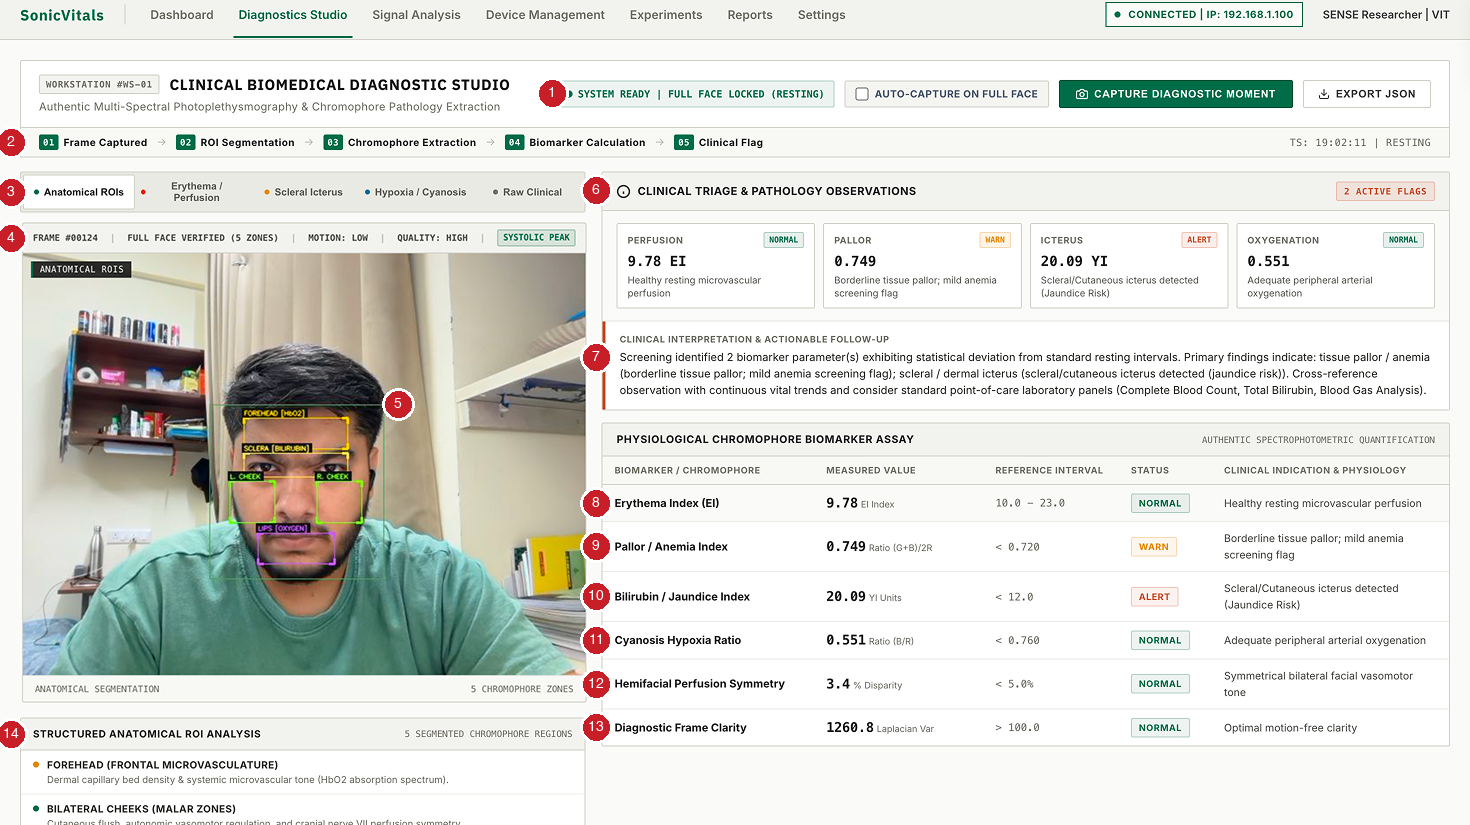
\includegraphics[width=\linewidth]{fig/diag.png}\end{center}

\begin{keybox}
\textbf{Idea.} Skin colour depends on chromophores: \emph{haemoglobin} (red, perfusion), \emph{deoxy-haemoglobin} (bluish),
\emph{bilirubin} (yellow), \emph{melanin} (brown). Ratios of mean R, G, B in chosen face regions give simple
\textbf{colorimetric indices}. They are \textbf{exploratory screening indicators, not diagnoses}: they depend strongly on lighting,
camera white balance and skin tone, and were not validated against blood tests.
\end{keybox}

\begin{labels}
\lab{1}{Status and controls.} Shows that the face gate passed. \emph{Auto-capture} grabs a frame automatically when the gate
passes. \emph{Export JSON} saves all values.
\lab{2}{Processing steps 01--05.} (01)~sharpest gated frame $\rightarrow$ (02)~five ROIs placed relative to the face box
$\rightarrow$ (03)~mean R, G, B per ROI $\rightarrow$ (04)~index formulas $\rightarrow$ (05)~compare with software reference
ranges (NORMAL / WARN / ALERT).
\lab{3}{View tabs.} Switch between the ROI view and false-colour heat maps (OpenCV colour maps) of each index over the face:
erythema (R vs.\ G), yellowness (CIELAB $b^*$), cyanosis (B/R).
\lab{4}{Frame info strip.} Frame number of the captured frame, ``5 zones'' verified, and \emph{Motion / Quality} labels.
\emph{Viva note:} both labels came from the sharpness value only ($>100 \Rightarrow$ LOW / HIGH); motion itself was not measured.
\lab{5}{Five anatomical ROIs.} Boxes at fixed fractions of the face box: \textbf{Forehead} (perfusion), \textbf{Sclera} band across
the eyes (yellowness), \textbf{Left/Right cheek} (pallor and symmetry), \textbf{Lips} (cyanosis).
\lab{6}{Triage cards (2 active flags).} The four headline indices repeated as cards; ``2 active flags'' counts rows not NORMAL
(Pallor WARN, Icterus ALERT).
\lab{7}{Interpretation text.} Auto-generated sentence listing the flagged indices. \emph{Viva note:} the clinical wording (anemia,
jaundice risk, lab panels) has been toned down in the current build to ``in/out of software range''.
\lab{8}{Erythema Index, EI $=9.78$.} $\text{EI}=100\,(\log_{10}\bar R-\log_{10}\bar G)$ on the forehead (Dawson/Diffey style). More
blood means more green absorbed, so $R/G$ and EI rise. Here $R/G=10^{0.0978}\approx1.25$. 9.78 is NORMAL because the code's actual range was
8--23; the ``10.0--23.0'' printed in the table was a label mismatch (fixed in the current build).
\lab{9}{Pallor index $=0.749$.} $\text{PI}=(\bar G+\bar B)/(2\bar R)$ on both cheeks. Less haemoglobin (anaemia) means less
red, so PI rises. $0.749 > 0.72$ gives WARN.
\lab{10}{Jaundice / yellowness index $=20.09$.} $\text{YI}=100\,(\bar R+\bar G-2\bar B)/(\bar R+\bar G+\bar B)$ on the eye band.
Bilirubin absorbs blue, so yellow tissue has low $B$ and high YI. \emph{Viva note:} the band includes skin and eyebrows, and warm
room light lowers $B$, so ALERT here is most likely \textbf{lighting/skin tone}, not jaundice. This is the main limitation of
RGB colorimetry without a colour reference card.
\lab{11}{Cyanosis ratio $=0.551$.} $\text{CR}=\bar B/\bar R$ on the lips. Deoxygenated blood looks bluer, so CR rises; below 0.76
is in range.
\lab{12}{Hemifacial symmetry $=3.4\,\%$.} $100\,|\bar G_L-\bar G_R|/(\bar G_L+\bar G_R)$, the left/right cheek difference in green
(perfusion). Large asymmetry can also come from side lighting, so it is an observation only.
\lab{13}{Frame clarity $=1260.8$.} Variance of the Laplacian (see Dashboard item 4); $>100$ is accepted as sharp.
\lab{14}{ROI analysis list.} Text description of each region and why it was chosen (e.g.\ forehead: thin skin, dense capillaries,
little hair or motion).
\end{labels}

% =====================================================================
\section{Signal Analysis (inside the HR estimate)}
\begin{center}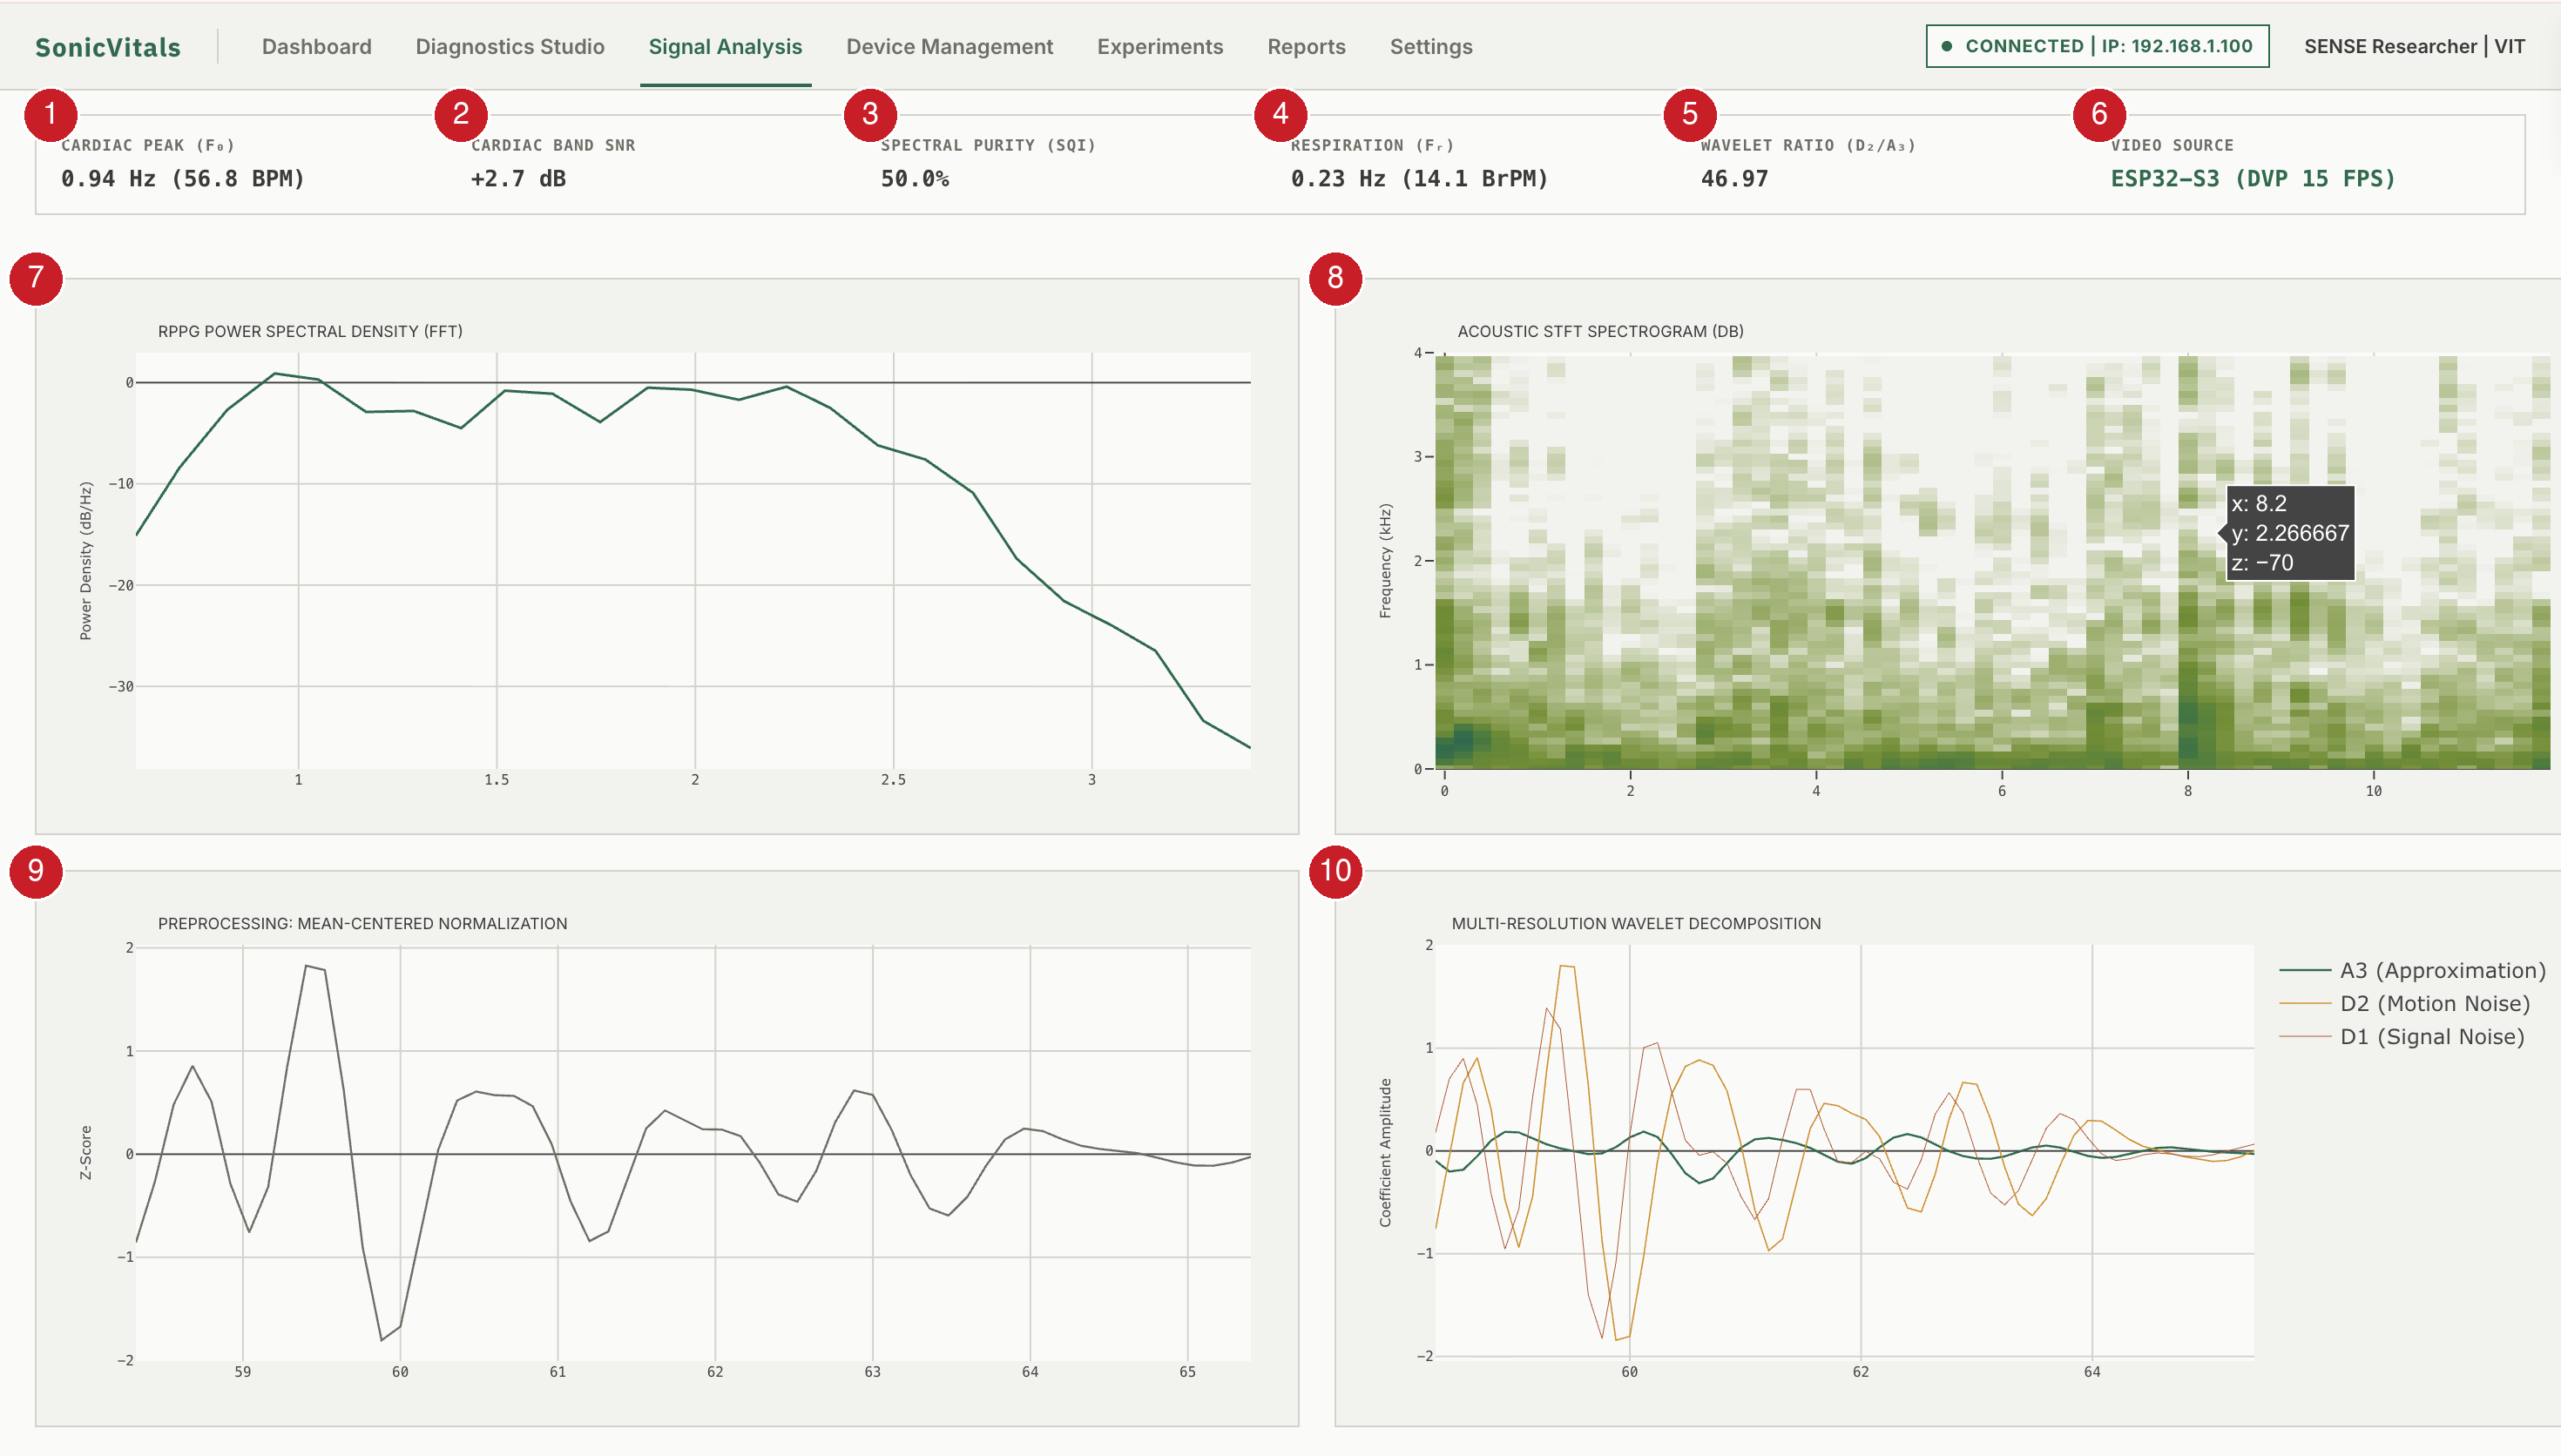
\includegraphics[width=\linewidth]{fig/sig.png}\end{center}

\begin{labels}
\lab{1}{Cardiac peak $f_0 = 0.94$ Hz (56.8 BPM).} Frequency of the highest point of the spectrum (item 7) inside 0.75--2.5\,Hz;
$\text{HR}=60\times f_0$. This screenshot is from a different moment than the Dashboard (97.3\,BPM), so the values differ.
\lab{2}{Cardiac band SNR $=+2.7$ dB.} First build: $10\log_{10}(P_\text{peak}/\text{median in-band power})$; $+2.7$\,dB means the
peak is only $1.9\times$ the typical level, i.e.\ \textbf{weak}. \textit{Current build} uses the standard de~Haan SNR: power within
$\pm0.1$\,Hz of $f_0$ and $\pm0.2$\,Hz of $2f_0$ (harmonic) divided by the remaining 0.5--4\,Hz power. HR is accepted only if
SNR $\geq 0$\,dB; pure noise passes this less than 5\,\% of the time.
\lab{3}{Spectral purity (SQI) $=50.0\,\%$.} Same quantity as Dashboard item 9; 50.0 is the clamped floor.
\lab{4}{Respiration $f_r = 0.23$ Hz (14.1 br/min).} Peak of the 0.15--0.40\,Hz respiratory spectrum; $60\times0.235=14.1$.
\lab{5}{``Wavelet ratio'' $D_2/A_3 = 46.97$.} Energy ratio $\sum D_2^2/\sum A_3^2$. \emph{Viva note:} it is \textbf{not} a true
wavelet transform. $A_3$ is a moving average of the BVP (about 1\,s window), $D_2$ is BVP $-\,A_3$ and $D_1$ is the first
difference. A 1\,s average almost cancels a 1\,Hz pulse, so $A_3$ is tiny and the ratio is large. The current build names this
honestly: trend / pulsatile / difference.
\lab{6}{Video source.} Which camera feeds the engine (ESP32-S3 over its parallel DVP camera bus). ``15 FPS'' was a fixed label.
\lab{7}{rPPG power spectral density.} \what how the pulse signal's power is spread over frequency (0.5--3.5\,Hz shown, in dB
relative to the maximum). \how \textbf{Welch's method}: split the signal into 50\,\%-overlapping segments, apply a Hann window,
take each FFT magnitude squared, and average. Averaging lowers the variance of the estimate. \textbf{Reading this plot:} the curve
is almost \emph{flat} from 0.9 to 2.3\,Hz, with several bumps within 1--2\,dB (0.94, 1.55, 1.9, 2.25\,Hz). So the 0.94\,Hz
``winner'' is barely ahead: a noisy recording. The straight segments come from coarse resolution: 128-sample segments at
15\,Hz give bins $15/128=0.117$\,Hz $=7$\,BPM apart. \textit{Current build:} 4096-point zero-padding plus parabolic interpolation
(sub-bin peak), peak tracking near the previous HR, and the SNR gate. The fall above 2.5\,Hz is the band-pass filter edge.
\lab{8}{Acoustic STFT spectrogram.} \what time (x, s) versus frequency (y, kHz), colour $=$ level in dB (white $=-70$\,dB floor,
dark green $=$ loud). \how \textbf{short-time Fourier transform}: FFT of short successive audio blocks (Web Audio analyser, FFT
512), one column per update. The tooltip $(8.2\text{ s},\,2.27\text{ kHz},\,-70\text{ dB})$ is a silent cell. \textbf{Reading:}
energy sits mostly below 1.5\,kHz (voice/room noise); vertical stripes (e.g.\ at 0 and 8\,s) are broadband clicks or speech.
Heart sounds (20--150\,Hz) would occupy only the bottom one or two rows (each row is about 90\,Hz wide), so the PCG is analysed
separately with a 25--400\,Hz filter and envelope autocorrelation (Dashboard item 12).
\lab{9}{Mean-centred normalisation.} The BVP in z-score units: $z=(x-\mu)/\sigma$. Removing the mean (DC) and scaling to unit SD
makes signals from different people, lighting and cameras comparable and is required before CHROM/FFT. Peaks $\approx$ beats;
the shrinking amplitude after 63 shows the signal fading (movement or light change).
\lab{10}{Multi-resolution decomposition.} Plots $A_3$ (slow trend, green), $D_2$ (pulsatile residual) and $D_1$ (first
difference) from item 5. $D_2$ carries the heartbeat oscillation; $A_3$ near zero shows little slow drift. Same viva note as
item 5: moving-average split, not a DWT.
\end{labels}

% Viva question bank, \input by SonicVitals_Viva_Guide.tex
\newpage
\section{Viva question bank}
{\small Short answers you can say out loud. \textbf{Bold} = the key point. Where a question is a trap, the answer says so.}

\newcommand{\qa}[2]{\par{\raggedright\bfseries Q.\ #1\par}\nopagebreak #2\par\vspace{3pt}}
\newcommand{\qgroup}[1]{\vspace{2pt}{\normalsize\bfseries\color{acc}#1}\par\vspace{1pt}}

\begin{multicols}{2}
\footnotesize
\setlength{\columnsep}{14pt}

% ---------------------------------------------------------------
\qgroup{A. Motivation and design choices}

\qa{Why not just use a phone or a webcam? The ESP32 image is poor.}
{\textbf{Not for image quality} (a phone is better): for (1)~\textbf{one clock} for camera and mic, so fusion is time-aligned;
(2)~\textbf{sensor control}: we lock exposure, gain and white balance after 3\,s, which phones and browser webcams keep
changing; (3)~a \textbf{chest microphone} for heart sounds, which a phone filming your face can't provide; (4)~a
\textbf{cheap, standalone node} with its own display and Wi-Fi. Trade-off accepted: 240$\times$160, about 8\,fps. The same software
also runs on a webcam (fallback mode), so a direct comparison is possible.}

\qa{What problem does the project solve?}
{Measuring vital signs \textbf{without touching} the person (no finger clip or chest strap): useful for burns, neonates, infection
control and continuous monitoring. We add a second modality (heart sounds) to check the camera estimate.}

\qa{What is novel here?}
{Not the algorithms (CHROM, Welch, PCG envelopes are published). The contribution is the \textbf{integration}: a
low-cost ESP32 node that streams time-synchronised video and audio, a camera/acoustic \textbf{fusion with an agreement gate},
\textbf{quality gating} that shows ``--'' instead of noise, and an honest study of what such a cheap sensor can and cannot do.}

\qa{Why ``SonicVitals''?}
{``Sonic'' for the acoustic (heart-sound) channel and ``Vitals'' for HR/RR; the system is multimodal: optical plus acoustic.}

\qa{Who would use it?}
{A research or screening prototype: telehealth kiosks, hostels and labs, low-resource clinics. \textbf{Not a medical device}; it
would need clinical validation and regulatory approval.}


% ---------------------------------------------------------------
\qgroup{B. Hardware}

\qa{Why the ESP32-S3?}
{Dual-core 240\,MHz Xtensa LX7, \textbf{8\,MB PSRAM} (frame buffer), a camera (DVP) interface, an \textbf{I$^2$S} interface for the
mic, built-in \textbf{Wi-Fi}, low cost. Two cores let audio and camera run in parallel without blocking.}

\qa{Which camera, and what is its limitation?}
{\textbf{GC2145} (2\,MP CMOS). It has \textbf{no hardware JPEG encoder}: the driver rejected JPEG mode, so we capture RGB565 and
compress in software (quality 60, about 5\,kB per frame). That limits us to about 8\,fps over Wi-Fi.}

\qa{Why the INMP441 microphone?}
{A digital I$^2$S MEMS mic: 24-bit output, so no analogue amplifier or ADC noise, and it is cheap and small.
\textbf{Limitation:} its response falls off below about 60\,Hz, while heart sounds are 20--150\,Hz, so it must be pressed on the
chest; in air the heart sounds are weak.}

\qa{What is the OLED for?}
{An SSD1306 128$\times$64 display over I$^2$C (GPIO47 SDA / 48 SCL, address 0x3C). It shows HR/RR/status sent back by the host and
the node's IP address, so the device is usable without the dashboard.}

\qa{Why couldn't you use USB for everything?}
{The board has one USB port, wired to a CH340 USB-to-serial chip on \textbf{GPIO43/44}. The mic's I$^2$S clock lines were on
the same pins, so with the mic on, the serial link died (verified). Also the CH340 was unreliable above 1\,Mbaud. So we stream
over \textbf{Wi-Fi}; USB is only for flashing and power.}

\qa{How is it powered? Power consumption?}
{5\,V over USB (laptop or power bank). \textbf{Power was not yet measured}; planned with a USB power meter (Table III of the paper). Do not
quote a number you haven't measured.}

\qa{Why PSRAM?}
{A frame ring buffer (24 slots $\times$ 16\,kB $\approx$ 3\,s) absorbs Wi-Fi stalls, so frames are not lost when the hotspot
briefly slows down.}


% ---------------------------------------------------------------
\qgroup{C. Firmware and communication}

\qa{How is the firmware organised?}
{FreeRTOS tasks: \textbf{audio task on core 0} (reads I$^2$S DMA, filters, queues blocks), \textbf{camera task on core 1}
(captures at a fixed 8\,fps, JPEG-encodes, puts frames in the PSRAM ring), and the main loop sends data, reads host commands and
updates the OLED.}

\qa{How are camera and audio synchronised?}
{Every frame and audio block carries a \textbf{microsecond timestamp from the same ESP32 clock} (\texttt{esp\_timer}) plus a
sequence number. The host analyses by timestamp, not arrival time, so network delay doesn't matter.}

\qa{Why TCP and not UDP?}
{A lost UDP packet would corrupt a JPEG frame. TCP guarantees order and delivery. Latency isn't critical because data is
timestamped at capture.}

\qa{Why not Bluetooth?}
{BLE throughput (tens of kB/s in practice) is too low for video plus audio; Wi-Fi gives about 70\,kB/s on a phone hotspot,
which is enough.}

\qa{What does the protocol look like?}
{Text lines: \texttt{<<HELLO:...>>}, \texttt{<<FRAME\_START:seq,t\_us,len>>} + base64 JPEG + \texttt{<<FRAME\_END>>},
\texttt{<<AUDIO:seq,t\_us,n,data>>}, \texttt{<<STAT:...>>} (fps, drops). Downlink \texttt{<<VITALS:HR,RR,SpO2,Q,STATUS>>} to the
OLED. The length field and sequence numbers detect corrupt or missing data.}

\qa{Why base64, which adds 33 \%?}
{It keeps the stream as plain text lines, so the parser can always re-synchronise at the next \texttt{<<} marker and it is easy to
debug. The cost is $4/3$ bandwidth; binary framing is future work.}

\qa{Why send JPEG and not raw pixels?}
{Raw: $240\times160\times2 = 76.8$\,kB per frame, 614\,kB/s at 8\,fps, far above the link. JPEG is about 5\,kB.
Downside: compression removes some of the tiny colour changes (McDuff et al., 2017).}

\qa{Why decimate audio from 16 kHz to 4 kHz?}
{Bandwidth: 16\,kHz $\times$ 2 bytes $=32$\,kB/s (43\,kB/s in base64) would starve the video. Heart sounds are below 400\,Hz, so
4\,kHz (Nyquist 2\,kHz) keeps them. A \textbf{63-tap FIR low-pass} filter runs first to prevent \textbf{aliasing}.}

\qa{Why lock exposure, gain and white balance?}
{Auto-exposure changes brightness every few frames, a change much larger than the pulse (0.1--1\,\%). After 3\,s of settling,
we freeze them so colour changes come from the skin, not the camera.}

\qa{How does the laptop find the board?}
{The node joins the phone hotspot and announces \texttt{sonicvitals.local} (mDNS); the host also scans the /24 subnet for port
3333. If no network is configured, the node becomes an access point (\texttt{SonicVitals-Node}, 192.168.4.1).}

\qa{How did you verify the link quality?}
{Measured over 30\,s: \textbf{8.0\,fps}, frame-timing jitter \textbf{0.4\,ms}, \textbf{0} dropped or corrupt frames, \textbf{0} audio
blocks lost (sequence numbers prove it).}


% ---------------------------------------------------------------
\qgroup{D. rPPG theory and signal processing}

\qa{What is photoplethysmography?}
{Measuring blood-volume changes optically. In a pulse oximeter a LED shines \emph{into} the finger; \textbf{remote} PPG uses
ambient light and a camera at a distance.}

\qa{Why does skin colour change with the heartbeat?}
{Each beat pushes blood into the capillaries; haemoglobin \textbf{absorbs green light strongly} (less red), so reflected green
dips slightly in systole. The change is about 0.1--1\,\% of the brightness.}

\qa{How can a change below 1 grey level be measured?}
{By \textbf{averaging thousands of pixels}: random noise falls as $1/\sqrt{N}$, while the pulse is common to all skin pixels and
survives.}

\qa{Why the forehead and cheeks?}
{Thin skin, dense capillaries, little hair, and relatively still. Forehead plus both cheeks gives more pixels than the forehead
alone, so lower noise. Beard and eyebrows are avoided.}

\qa{Explain CHROM.}
{Normalise R, G, B by their means (removes light intensity). Build $X=3R_n-2G_n$ and $Y=1.5R_n+G_n-1.5B_n$; both contain the
motion/specular part, so $S=X-\alpha Y$ with $\alpha=\sigma_X/\sigma_Y$ \textbf{cancels it} and keeps the pulse (de Haan \& Jeanne
2013).}

\qa{Why not just the green channel?}
{Green has the strongest pulse but also all the lighting and motion changes. CHROM is more robust; we keep green as a baseline
for comparison (ablation).}

\qa{CHROM vs POS vs deep learning?}
{POS (Wang 2017) is a similar projection; either works. Deep models (DeepPhys, PhysNet) can be more accurate but need large
training sets and a GPU, and may not generalise to a new low-quality camera. CHROM needs no training.}

\qa{Why band-pass 0.75--2.5 Hz?}
{0.75--2.5\,Hz $=$ 45--150\,BPM, the expected range. It removes breathing ($<0.4$\,Hz) and high-frequency noise.
\textbf{Limitation}: HR below 45 (athletes) would be missed.}

\qa{Why Butterworth, and why filtfilt?}
{Butterworth has a \textbf{maximally flat passband} (no ripple distorting amplitudes). \texttt{filtfilt} runs it forwards and
backwards, giving \textbf{zero phase shift}, so peaks are not delayed.}

\qa{Why resample to 15 Hz?}
{Frames arrive at uneven times over Wi-Fi; the FFT needs uniform samples. Each frame is placed at its capture timestamp and
linearly interpolated onto a uniform grid.}

\qa{Is 8 fps enough? (Nyquist)}
{The sampling rate must exceed twice the highest frequency. HR up to 150\,BPM is 2.5\,Hz, which needs $>5$\,fps; 8\,fps gives
4\,Hz Nyquist. Enough for HR, not for fine waveform shape or HRV.}

\qa{What is Welch's method and why use it?}
{Split the signal into 50\,\%-overlapping segments, apply a Hann window, average the periodograms. Averaging \textbf{reduces
the variance} (noise) of the spectrum compared with a single FFT.}

\qa{Why a Hann window?}
{Cutting a signal abruptly causes \textbf{spectral leakage} (power smeared into other bins). The Hann window tapers the ends and
reduces leakage.}

\qa{What is the frequency resolution?}
{$\Delta f=1/T$. A 10\,s window gives 0.1\,Hz $=6$\,BPM. \textbf{Zero-padding} (FFT length 4096) only interpolates the spectrum;
\textbf{parabolic interpolation} through the peak and its neighbours then estimates the peak between bins.}

\qa{Why wait 10 s before showing HR?}
{To get about 8--15 beats and a usable frequency resolution. Shorter windows give unstable peaks. The analysis buffer is 30\,s.}

\qa{How do you know a reading is good? (SNR)}
{The de Haan \textbf{SNR}: power near $f_0$ and its harmonic $2f_0$ divided by the rest of 0.5--4\,Hz, in dB. HR is accepted only if
SNR $\geq 0$\,dB. We set this threshold by testing pure noise: it passes in fewer than 5\,\% of cases.}

\qa{What is spectral concentration $Q$?}
{The share of in-band power within $\pm0.1$\,Hz of the peak. High $Q$ means one clear peak. It is used as the camera's fusion
weight.}

\qa{What happens when the person moves briefly?}
{Gaps up to \textbf{2\,s} are bridged by interpolation, so the estimate continues. Longer breaks restart the 10\,s buffer while the
last value is \textbf{held} (marked ``HELD'') for up to 15\,s.}

\qa{How do you stop the HR jumping between peaks?}
{\textbf{Peak tracking}: if a peak within $\pm12$\,BPM of the last accepted HR has at least half the power of the highest peak,
it is kept. The displayed value is a median of the last 3 estimates followed by an exponential moving average (EMA).}

\qa{How does face detection work?}
{\textbf{Viola--Jones Haar cascade}: Haar-like rectangle features computed quickly from an integral image, chosen by AdaBoost,
arranged in a cascade that rejects non-faces early. Fast on a CPU. The box is smoothed to reduce jitter.}

\qa{Why not a deep face detector (MediaPipe)?}
{Haar is light and real-time on a laptop CPU. MediaPipe Face Mesh would track landmarks better under head turns: \textbf{future
work}.}

\qa{What are the five face-gate tests?}
{Not touching the edges; size 20--88\,\% of the frame width; aspect ratio 0.65--1.30 (not turned); all ROIs inside the frame;
enough light and similar left/right brightness. Frames that fail are not used.}

\qa{Two faces in the frame?}
{The largest face is used. Multi-person tracking is future work.}


% ---------------------------------------------------------------
\qgroup{E. Respiration, SpO$_2$ and HRV}

\qa{How do you get the breathing rate from a face?}
{Breathing modulates the skin signal (venous return, chest and head movement, light angle): \textbf{respiratory-induced intensity
variation}. Band-pass green 0.15--0.40\,Hz (9--24 breaths/min), take the spectral peak. Needs 15\,s and a clear peak
($\geq 50\,\%$ of the low-frequency power), otherwise ``--''.}

\qa{Can a camera measure SpO$_2$?}
{Only roughly. Pulse oximeters use the \textbf{ratio of ratios} $(AC/DC)_{red}/(AC/DC)_{IR}$; our camera has no infrared, so we
use red/blue as a proxy. It needs \textbf{calibration} against a reference oximeter ($\text{SpO}_2=A-B\cdot R$). Without that file,
the dashboard shows only the uncalibrated ratio.}

\qa{What is HRV and how do you measure it?}
{Beat-to-beat variation of the inter-beat interval (IBI). RMSSD $=\sqrt{\text{mean}(\Delta IBI^2)}$. We compute it from heart-sound
beat times and need $\geq 20$ clean intervals. At 8\,fps the camera's time resolution (125\,ms) is too coarse for HRV.}

\qa{What is LF/HF?}
{The ratio of HRV power at 0.04--0.15\,Hz to 0.15--0.4\,Hz, used as a sympathovagal-balance (stress) index. It needs several
minutes of accurate beats, so we \textbf{removed} the stress card (it was a placeholder).}


% ---------------------------------------------------------------
\qgroup{F. Heart sounds (PCG)}

\qa{What are S1 and S2?}
{S1 (``lub''): mitral and tricuspid valves closing at the start of systole. S2 (``dub''): aortic and pulmonary valves closing at the
end. Main energy is about 20--150\,Hz.}

\qa{How do you get HR from sound?}
{Band-pass 25--400\,Hz, resample to 1\,kHz, \textbf{Shannon energy} envelope $-x^2\log x^2$ smoothed over 20\,ms, then
\textbf{autocorrelation}: the first strong peak at lag $\tau$ (0.4--1.33\,s) is one beat period, so $\text{HR}=60/\tau$.}

\qa{Why Shannon energy and not just $x^2$?}
{$x^2$ is dominated by the loudest peaks. Shannon energy emphasises \textbf{medium-intensity} sounds and suppresses both low
noise and very high spikes, giving a cleaner envelope.}

\qa{Why autocorrelation instead of peak picking?}
{It uses the \textbf{periodicity of the whole window}, so it is robust to a few missed or extra peaks; it does not need to label
S1 vs S2.}

\qa{What is $\rho$?}
{The autocorrelation value at the beat lag (0--1): how periodic the sound is. Below 0.3, the acoustic HR is not reported.}

\qa{Did the heart-sound channel work?}
{\textbf{Honestly: weakly.} In air, 99.5\,\% of the audio power was below 25\,Hz and $\rho$ stayed $\leq 0.18$, because the
INMP441 cuts off around 60\,Hz. It needs firm chest contact or a stethoscope-coupled mic: \textbf{future work}.}


% ---------------------------------------------------------------
\qgroup{G. Fusion}

\qa{How do you fuse camera and sound?}
{Quality-weighted mean $(w_oHR_o+w_aHR_a)/(w_o+w_a)$, with $w_o=Q$ (camera) and $w_a=\rho$ (sound). \textbf{Agreement gate:} only if
they differ by $\leq 8$\,BPM; otherwise use the better channel and flag ``CONFLICT''.}

\qa{Why an agreement gate?}
{Averaging a correct value with a wrong one gives a wrong answer. If two independent sensors disagree, one is failing, so we
don't average.}

\qa{Why 8 BPM?}
{Slightly above the AAMI tolerance ($\pm5$\,BPM) to allow for each channel's own error. It is a tunable parameter, to be
re-tuned on development data.}


% ---------------------------------------------------------------
\qgroup{H. Colour indices (Diagnostics Studio)}

\qa{Can a camera detect jaundice or anaemia?}
{It can give \textbf{screening hints}. Research (e.g.\ BiliScreen) used colour-calibration cards and controlled light. Ours are
\textbf{uncalibrated and exploratory}; lighting and skin tone change them a lot.}

\qa{Your screenshot says jaundice ALERT. Do you have jaundice?}
{\textbf{Trap.} No: warm room light lowers blue, and the eye band includes skin and eyebrows, which raises the yellowness
index. It shows exactly why calibration is needed.}

\qa{Why log in the erythema index?}
{By the Beer--Lambert law, absorbance is logarithmic in reflectance, so $\log R - \log G$ tracks haemoglobin absorption roughly
linearly.}

\qa{What is the Laplacian variance?}
{A sharpness measure: the variance of the 2nd-derivative image. Blurred frames have weak edges and a low value; we pick the
sharpest frame for colour analysis.}

\qa{How would you make colour indices reliable?}
{A colour reference card in the frame, fixed lighting, white-balance correction, and validation against lab tests (bilirubin,
haemoglobin) with ethics approval.}


% ---------------------------------------------------------------
\qgroup{I. Validation, accuracy and limitations}

\qa{How accurate is your heart rate?}
{\textbf{Not yet validated} against a reference device; we will not claim a number we haven't measured. Validated so far: the
algorithms on synthetic signals (31 automated tests), and the streaming link (8\,fps, 0 loss). Planned: ECG chest strap as
reference.}

\qa{How will you validate it?}
{Simultaneous ECG chest strap (HR, R--R intervals), finger oximeter, metronome breathing; conditions at rest, talking, small
motion, low light, different distances; 30\,s windows; \textbf{MAE, RMSE, Pearson $r$}, \textbf{Bland--Altman} bias and 95\,\% limits
of agreement, and the \textbf{AAMI EC13} criterion (error $\leq 5$\,BPM or 10\,\%).}

\qa{What is a Bland--Altman plot?}
{Difference (device $-$ reference) against their mean. The \textbf{bias} is the mean difference; the \textbf{limits of agreement}
are bias $\pm1.96$\,SD. It shows agreement; correlation only shows that two values move together. With several windows per
person, the repeated-measures version is used.}

\qa{Why not just use correlation?}
{Two methods can correlate perfectly yet differ by 10\,BPM. Agreement needs bias and limits (Bland \& Altman, 1986).}

\qa{Why split development and test participants?}
{Thresholds (SNR gate, $\Delta$, RR gate) are tuned on development participants only, so test results are not biased by
tuning.}

\qa{Main limitations?}
{\textbf{Motion} and \textbf{lighting changes}; low resolution, 8\,fps and JPEG compression; \textbf{skin tone} (more melanin means a
weaker pulse signal, a known bias in rPPG); beard and hair covering ROIs; weak heart sounds through air; no clinical
validation yet.}

\qa{Does skin tone matter?}
{Yes. Melanin absorbs light and reduces the pulse amplitude, so SNR is lower for darker skin (Nowara et al., 2020). The SNR gate
avoids wrong numbers but may show ``--'' more often. Diverse participants are needed.}

\qa{What about fluorescent light flicker?}
{Mains lighting flickers at 100\,Hz. With 8\,fps sampling it can alias into the low-frequency band as a fake peak. Locking the
exposure and using daylight or DC LED light reduce it.}

\qa{What if I show it a photo of a face?}
{The face detector will find it, but a photo has no pulse: the spectrum is noise, the SNR stays below the gate, and HR shows
``--''. (A photo under flickering light could still pass occasionally; liveness detection is future work.)}

\qa{Why did your earlier screenshot show 97 BPM and another 57 BPM?}
{Different moments; and in that first build there was no quality gate, so noisy windows were still displayed. The current
build only shows estimates that pass the SNR gate.}

\qa{Your HRV was exactly 45.0 and stress exactly 50.0. Why?}
{\textbf{Trap; be honest.} In the first build those were placeholder formulas driven by the quality score; with quality at its
floor (50) they gave 45.0 and 50.0. I found this, removed them, and replaced HRV with real RMSSD from heart sounds.}

\qa{What is the latency?}
{About 10\,s for the first estimate (buffer), then an update every 2\,s on the dashboard and every 1.5\,s to the OLED.}


% ---------------------------------------------------------------
\qgroup{J. Software}

\qa{Software stack?}
{Firmware: Arduino core on ESP-IDF/FreeRTOS, built with PlatformIO. Host: Python, Flask, OpenCV, NumPy/SciPy. Frontend:
HTML/CSS/JavaScript with Plotly charts, polling the Flask JSON API.}

\qa{Why process on the laptop instead of on the ESP32?}
{Face detection, CHROM and spectral analysis in Python are easy to develop, debug and change. The ESP32 could run a simpler
version (e.g.\ fixed ROI plus FFT): \textbf{edge processing} is future work and would also remove the video stream.}

\qa{How do you record data for analysis?}
{The ``Experiments'' tab starts a session: \texttt{frames.csv} (timestamps, ROI colour, gate), \texttt{audio.wav},
\texttt{estimates.csv}, \texttt{meta.json}. \texttt{analysis/evaluate.py} replays them offline with the \textbf{same} DSP code.}

\qa{How did you test the software?}
{31 automated \texttt{pytest} tests with synthetic signals of known HR/RR (e.g.\ 52/78/128\,BPM within 2\,BPM), protocol parsing,
gap bridging, noise rejection, and a node simulator that imitates the ESP32 stream.}

\qa{Privacy and security?}
{Everything stays on the local network; nothing goes to the cloud; video is saved only during an explicit recording. Limitation:
the TCP stream is not encrypted (WPA2 only protects the Wi-Fi link).}


% ---------------------------------------------------------------
\qgroup{K. Future work}

\qa{What would you improve first?}
{(1)~A validation study with an ECG reference; (2)~compute ROI colour means \textbf{on the ESP32 from raw pixels} before JPEG
(avoids compression loss); (3)~a stethoscope-coupled or contact mic; (4)~a landmark face tracker; (5)~an IR camera/LED for SpO$_2$;
(6)~edge processing and a battery.}

\qa{Could this become a product?}
{After clinical validation, IEC 60601 electrical-safety testing and regulatory approval (CDSCO in India) as a medical device. Today
it is a research prototype.}

\end{multicols}


\end{document}
